
Whenever tasks become more extensive and complex, systems react with division of work and specialization. Driven by chance and selection, we call this process evolution. By subdividing into smaller, less complex tasks, large processes can be distributed and processed in parallel, and at the same time the executing components are more efficient because they have to cover less noise, peripheral cases and side aspects. We can observe this development on different scales in computer science. At the hardware level, computations are distributed from general-purpose CPUs to GPUs, digital signal processors (DSPs) or other adapted hardware, and the concrete hardware logic is abstracted from the programme logic to be executed. At the software level, components are separated both vertically, i.e. between business logic, language runtime environment and operating system services, and horizontally, i.e. between components of the different levels of independence. 

Besides improved efficiency and scalability, compartmentalization has also a major advantage when it come to security. Separation of concerns and minimization of trust assumptions are core concepts in defense in depth for cloud deployments. But again they are likewise seen on the scale of single machines. A cloud deployment consisting of one big trust zone protected by a perimeter is the large scale equivalent of a monolithic kernel, with unrestricted memory access among all kernel space processes. The problem with this is clearly evident in monolithic Unix kernels. Despite various measures to prevent unauthorized memory access (control flow integrity, data execution prevention) or to make it more difficult to exploit security vulnerabilities (address space layout randomization, stack canaries), according to statistics of the NIST\cite{nvd} the number of vulnerabilities in the kernel ecosystem is still increasing. An analysis of the NIST National Vulnerability Database in \cite{mckee2022novel} looked at the reasons for critical vulnerabilities over the last 5 years and concluded that 34\% of them were due to lack of storage security, and another 43\% were due to lack of compartimentalization. The authors also pointed out, that these vulnerabilities could have been prevented if essentially independent processes could not access shared memory but that however the so-called least-privilege policy is not enforced by the Linux kernel or other big open source projects as OpenSSL or the Apache Server. 
Similarly, as the authors report in \cite{kirth2022pkru}, the majority of known vulnerabilities in Windows, Chrome and the Android Open Source Project (AOSP) can also be traced back to insecure memory access. 

So obviously it is desirable to have compartmentalization and data locality enforcement not only in cloud setting but also in the kernel itself. The downside of distributing computation to independent component is however, that it requires manual adaptation and complicates development and testing. It also 


\begin{itemize}
    \item[State of things]
    \item Second: There are generally two large trends \means distribution + heterogeneity vs need for security+safety+verification 
    \item In both of this cases, the original single-core/thread/address space version had its advantages. Mostly ease of communication, ease of development and testing, known environment. And in both of this cases migration to a separated, concurrent, distributed setup comes at a cost. 
    \item downside \means development more difficult, hard to verify, etc pp
    \item on the other hand security doesn't necessarily suffer with distribution, because at least in theory compartmentalization of large applications and composition of smaller, components with limited access rights is a security in depth approach, trend in DevSecOps
    \item One particular instance of that dilemma is the kernel itself. Unix based operating systems have long been based on a monolithic kernel. 
    
    \item[Problem with that]
    \item On the one hand, distribution facilitates isolation \means good
    \item On the other hand, distribution comes with concurrency and increased complexity of programming (incl. new layer of abstraction) and they are the "natural enemy" of verification
    \item another issue, in particular when systems need to be secure is the adaptation overhead to new execution scenarios


    \item Approache so far: ...
    \item we can see the struggle is real 
    \item[Process Isolation]
    \item Operating systems and kernel designs that already isolate kernel components just as normal processes
    \item \todo[inline]{Check HAKC\cite{mckee2022preventing}, Endokernel\cite{im2021endokernel}}
    \item memory isolation techniques as HW implementation 
    \item virtualization 
    \item \means mostly specific software or even HW solution i.e. existing sw. must be adapted, deployment tied to specific HW, testing and development tied to setup, SW solutions come with aditional layers of SW obviously that needs to be trusted.
    \item citation on TEEs and new alternative \url{https://dl.acm.org/doi/abs/10.1145/3453933.3454024}
    \item \todo[inline]{ Check \cite{9973038}: Combined approach using HW protection techniques, compile time analysis, model checking, and compiler runtime measures for protection. Probably cites a lot of approaches.}
    \item[Developing distr. systems]
    \item cite approaches to verify OSes
    \item cite e.g. Model Checking for Distributed Systems 
    \item maybe also cite various approaches towards memory safety and isolation (VMs, containers, secure enclaves, memory protection keys,...? )
    
    \item[Our approach]
    \item Certain costs are unavoidable when program parts are isolated and can no longer communicate directly and via shared memory. The costs of manually adapting to different isolation mechanisms are not among them. The classic approach to separating concrete run-time implementations from program logic is compilers. They allow the programmer to define and test the logic within specific programming models and automatically translate and add to them to fit the chosen runtime environment and architecture.
This work will therefore also be based on an existing compiler. This compiler is called Ohua. Ohua works on subsets of high-level languages such as Python or Rust. Instead of machine code, Ohua extracts a dataflow program from the input, introducing two main abstractions, the notion of an independent node and the notion of communication edges, and replaces them with the corresponding implementations for different runtimes.  

    \item The idea of this work is to use and extend Ohuas capabilities for program transformation. We want to be able to extract isolated components from a shared memory program suitable for unikernels and automatically derive the code to deploy them in a microkernel setting. 

    \item Therefor we need to understand 

    \item A good example case for this purpose is a server applications. They are quasi-ubiquitous in distributed applications and consist of various components, in particular the data backend, the TCP/IP-Stack and a network driver, that should be isolated from each other for security reasons. 
    
    \item develop and verify the sequential, local code \means have verified transformations applied \means get a verified distributed program with isolation boundaries inserted automatically
    \item classical scenario on OS level is a NW stack. It connects user App to the outside world, uses different system services and in particular (nw) device drivers which is relevant because device drivers are notorious for bugs
\end{itemize}

Actual Problem description
\begin{itemize}
    \item what we have is a library called smoltcp, that implements the network stack in userspace \means it can be used in a unikernel setting, where such system services are not part of the kernel
    \item what we want is the ability to compile applications build with smoltcp to run in a microkernel setting in particular in the M$^3$ hw-os system
    \item Why is this interesting:
    \begin{enumerate}
        \item Transformation to message passing: In it's current state, smoltcp actually combines the TCP/IP stack and an interface to the actual physical layer. The according parts of the library are coupled via shared references and invoke each other via normal function calls. This works well in unikernels, as well as in monoliths (implemented in user space vs. kernel space respectively). In a microkernel, we might want to separate this two functionalities to use and scale them independently. This requires components to interact not vie function calls and shared references but via IPC. SO one aspect of the problem is to investigate which constraints the isolation of components imposes on the code and which transformations achieve a compatible structure. Exmpl: We can not call functions with mutable references any more because the sematics of such calls change, when components are separated and objects are serialized upon invocation.
        \item Local State: Smoltcp is a good example for an application with interacting states. From a bird's eye view we can basically distinguish three states, the server application holding e.g. requests currently to process, the network stack holding for example socket states and the network interface abstraction \todo[inline]{I don't think thats a stateful thing, it's basically a source/sink abstraction to the system}. 
        
        \todo[inline]{describe a) the state locality problem i.e. write the code such that no internal function will try to access another components state outside the 'flow' b) rewrite it such a way, that Ohua identifies the components we want}
        Take the example in  ... 
        So the question is, can we a) identify all syntactic constructs that lead to states being transferred in the resulting DFG and b) identify code transformations to avoid this (on the level of input code)
        \item Compile from Uni- to Microkernel \question{$M^3$ already is a Microkernel using smoltcp as a userspace service, so how to describe exactly what's the point here?}
        \item True, but we do not target OS1 \means OS2 but only OS1 mono/unikernel \means OS1 microkernel \textcolor{gray}{Transpile to another Operating System: Current Ohua integrations \todo[inline]{Check if this hold historically} produced concurrent version of a sequential input program both running on in basically the same runtime environment i.e. the OS interface and standard components of the language (e.g. the Rust standard library). This is not the case for M3. M3 does (to the date this work is written) not support the Rust standard library. }
        \todo[inline]{As it supports libc, and smoltcp doesn't need std this could be no big thing for now. However it is a general problem to consider, also with respect to cloud environments, that (out-of-scope) parts of the compiled software use functions, that rely on system interfaces being present or having a particular semantic, e.g. opening files, writing to stdout/err, trying to access sytem services as time or randomness}
        \item Extending the Rust subset of Ohua: Ohua is currently lacking some general as well as Rust specific language constructs. Most importantly compiling a condition guarded loop (\code{while} or \code{do-while}) is currently not supported. Further Ohua does currently not accept structs, impl functions and trait implementations in the compile scope (i.e. they can be used only in the called libraries). So another goal is to describe and implement code transformations (or, if necessary, remaining restrictions) to accept struct and impl definitions. 
        
        \item Exemplify Usage: The last point is to demonstrate the domain knowledge required from the programmer. Ohua obviously can not tell, for any two structs or modules of smoltcp and applications using it, if they should end up in the same service or not. The level and lines of separation have to be provided by the programmer. Specifically the composition of function calls in the compilation scope determines the structure of the derived DFG. \todo[inline]{example}
    \end{enumerate}
   
\end{itemize}
    \begin{figure}[H]
    \centering
    
    \begin{subfigure}[b]{0.6\textwidth}
         \centering
         \begin{minted}{rust}
   fn somefun() -> i32 {
       let mut mStruct = MS::default();
       let i = mStruct.f();
       let j = mStruct.g();
       calculate(i,j)
   }       
            \end{minted}
         \caption{Multiple calls to a struct}
         \label{multCalls}
     \end{subfigure}
     %\hfill
     \par\bigskip
     \begin{subfigure}[b]{0.6\textwidth}
         \centering
         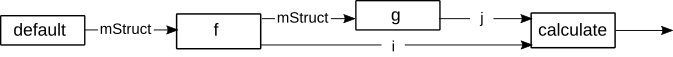
\includegraphics[width=\textwidth]{figures/graph_state_moved.png}
         \caption{Resulting data flow graph}
         \label{DFGStateMoved}
     \end{subfigure}
    \par\bigskip
     \begin{subfigure}[b]{0.6\textwidth}
         \centering
         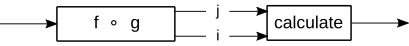
\includegraphics[width=0.6\textwidth]{figures/graph_state_not_moved.png}
         \caption{Target data flow graph}
         \label{DFGStateNotMoved}
     \end{subfigure}
    \caption{}
    \label{fig:SimpleStateUseFigure}
    \end{figure}
    
    \todo[inline]{Explain the contingency from SharedMemory programming model, over M3 to Cloud deployment: maybe Mention in Intro, details in the background}
    Describe essential differences at: 
    \begin{itemize}
        \item Is it one program or do we compile/deploy different programs?  $\rightarrow$ are types known/inferable at compile time/do they have to be? $\rightarrow$ Do we compile for the same OS? \\
         $\Rightarrow$ points above have consequences e.g. 
        \item What are the constraints on types being passed (serializable, are \rust{dyn} allowed, are generics allowed, who takes care of compatibility in case of different OSs)? 
        \item What are other constraints for the programmer (e.g. using system specific interfaces for components) How much packaging does the Compiler have to do (e.g. assorting libraries to components)? 
        \item (How) do we need to handle errors/panics?(in a 'one program' scenario it's one panic to crash them all. How is it in M3? It's even more complex in 'really' distributed scenarios as there are different reasons components might not answer and even if they answer with an error we might have different strategies to handle.)
        \item Do we need to build in a shut down mechanism? 
        \item Can/Should the Compiler be able to detect system interaction and tailor them?        
    \end{itemize}
    
\todo[inline]{Important Point I don't know where to put yet and also needs elaboration:}
\note{The transformation we will extract from the rewriting process are to some degree actually extensions of Ohua programming model. The model currently already enforces 1) variables to be either used as state, or as variable i.e.\means no sending of states and 2) states from outside the loop scope to be only used once inside loop or recursion \means linearity inside loops. What is not enforced currently is, that states in general are used only once, i.e. outside loops or when created inside loops states can be used more than once \means so no linearity here.}

    

From the task definition
\begin{itemize}
    \item Implement the cloud-unikernel using SmolTCP, a well-established networking library -> Also schlicht eine Beispielanwendung mit smoltcp, die Anfragen an einen Key-Value-Store handelt. 
    \item Rewrite the unikernel, such that Ohua can compile it Derive and implement transformations to make state usage local to a single program location to provide isolation.
    \item Update existing M3 Backend
    \item Evaluate the approach in the (existing) setup of the YCSB key-value store benchmark along the performance-safety trade-off. 
\end{itemize}

\todo[inline]{Example Rust 4 Unikernel \cite{Rust4Unikernel}}
\todo[inline]{Formal Verification eg for L4 derivatives as motivation \cite{sL4Verf}}

\todo[inline]{Can I get e reference to Compositionality papers .. It would be awesome if we could get the link to \means "we transform a verified object into a verified category, i.e. composable, verified objects"}
